Proteins are key actors of biological processes inside cells. Rather
than carrying out tasks as single agents, they are part of dynamic
networks of protein-protein interactions (PPIs) \cite{Lin2017}. Such
networks underlie a variety of interdependent mechanisms, including
signal transduction, homeostasis control and stress responses, and 
play an important role in physiological and developmental
processes such as protein phosphorylation, transcriptional co-factor
recruitment and transporter activation \cite{Zhang2010PPI}.

\emph{Yeast-Two-Hybrid} technique (also known as 
\emph{two-hybrid screening} or \emph{Y2H}) is a commonly used 
technique to generate PPI networks. Figure \ref{Y2H}A
illustrates the biological basis of Y2H. The expression of a specific
reporter gene is activated by binding a DNA-binding Domain
(DB) and an Activation Domain (AD) of a Transcription Factor, which
in turn binds to an Upstream Activation Sequence (UAS). To evaluate
an interaction between two proteins, the Y2H approach fuses one protein
(known as \emph{bait}) to the DB domain and the other (known as 
\emph{prey}) to the AD. If the proteins interact, the reporter
gene expression is activated by the AD (Fig. \ref{Y2H}B). Otherwise,
if proteins fail to interact, the reporter gene is not expressed (Fig.
\ref{Y2H}C).

\begin{figure}[h]
\caption{\label{Y2H}Yeast-2-Hybrid offers an experimental approach
for constructing PPI networks.}
\centering
	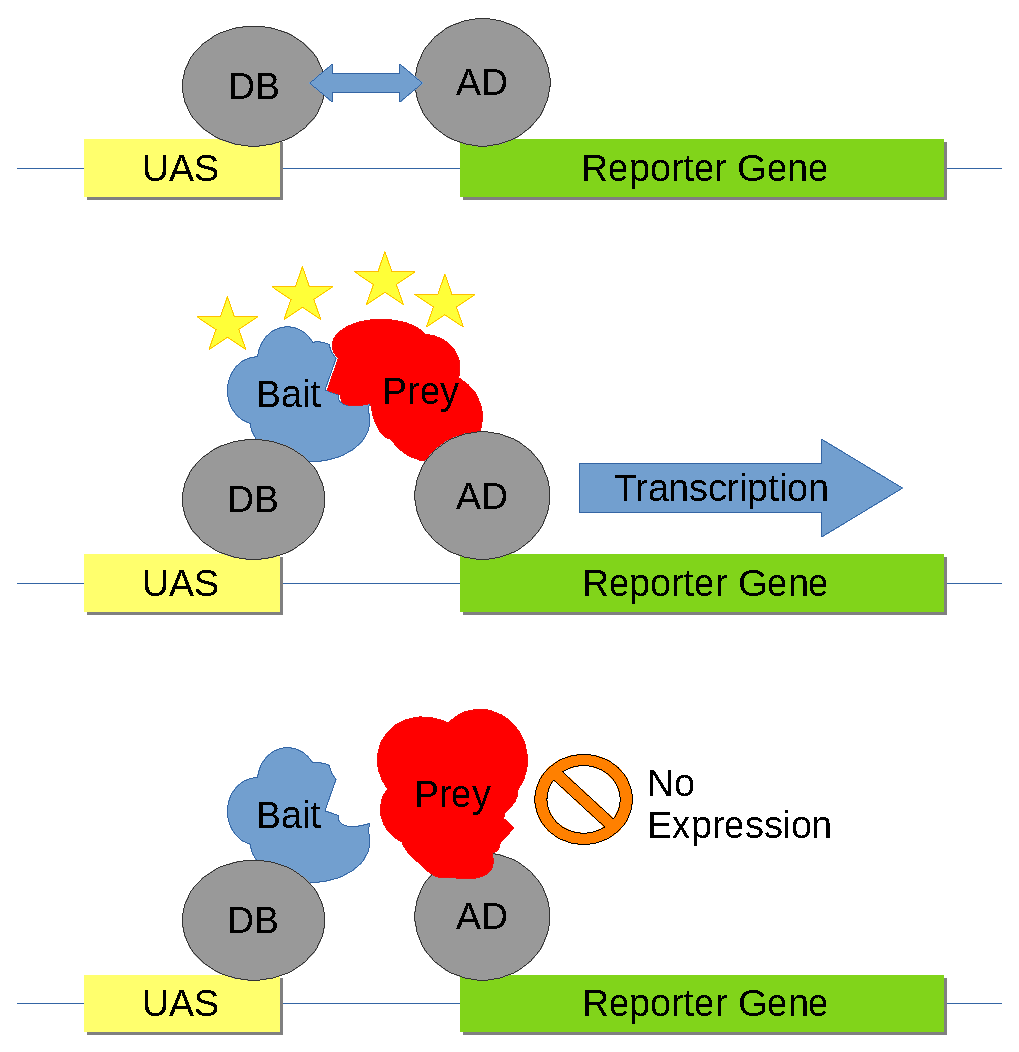
\includegraphics[width=0.7\columnwidth]{../Y2H}
\end{figure}

Based on the outcome of Y2H experiments, numerous networks
of interactions between proteins have been constructed \cite{Weimann2013Y2H,Rajagopala2015Y2H,Shokri2019TFY2H}.
However, identifying protein interactions through Y2H experiments is 
costly both in terms of time
and resources \cite{Laraia2015PPI,Macalino2018PPI}. For example, 
constructing a PPI network for an organism with 2000 unique 
proteins requires the above validation procedure to be repeated 
around 2 million times. Computational tools for predicting such 
interactions offer a cpst-effective alternative, especially for 
organisms that produce a large number of proteins.

Different methods for predicting interactions based on PPI networks have
been proposed \cite{Chang2016PPI,Chen2019PPI,Kotlyar2015PPI}. A first 
approach for predicting PPIs is based the triadic closure principle
(TCP), which states that the higher the number of common neighboring
nodes between two nodes, the higher the probability that they interact
\cite{Goldberg2003SmallWorld}. TCP is measured by counting the number 
of shared neighbors of a pair of nodes (denoted as A2), namely by raising the adjacency
matrix of the PPI network to the second power ($A_G^2$). 
However, previous studies show that TCP often falls short as it does 
not consider the structural and chemical properties of the proteins
\cite{Cannistraci2013Networks}, which are related to 
complementarity in charges and arrangement of atoms between pairs of proteins.

The work in \cite{Kovacs2019} introduces another network-based approach which predicts
an interaction between two proteins based on the number of paths
of length 3, in contrast to the number of paths of length 2, denoted as A2. 
The number of paths of length 3, denoted as A3, is computed by raising
the adjacency matrix of the network to the third power. Furthermore, the 
degree-normalized measure of A3, denoted as L3,  mitigates bias caused by
intermediate hubs within the paths of length 3. Using the measure of L3, 
the approach in \cite{Kovacs2019} outperforms previous methods for predicting
binary protein interactions for various organisms, including yeast (\emph{S. cerevisiae}),
Arabidopsis (\emph{A. thaliana}), worm (\emph{C. elegans}), fly (\emph{D. melanogaster}),
fission yeast (\emph{S. pombe}), mouse (\emph{M. musculus}) and humans.

This paper extends previous analyses by using handcrafted features (A2,
A3, L3) as well as learned representations of the proteins and their 
neighborhoods within the PPI networks in human and rice 
interactomes (\texttt{node2vec}) \cite{Grover_2016}. To evaluate the 
proposed approach, predictions of interactions are carried out 
using a supervised Machine Learning algorithm called \texttt{XGBoost} 
\cite{2016ChenXGB}. XGBoost is particularly useful since its gradient 
boosted decision tree model weighs the different features and 
establishes the importance of each feature. The main results of this paper 
show that adding the handcrafted features derived from the
network connectivity to the Machine Learning model improves the prediction
power of the models. This property can be assessed when looking at the their
importance in the model. The main contributions of this paper are twofold. 
First, a general framework for link prediction in non-directed networks is 
introduced. Second, two applications of this framework to biological networks 
with a structural insight are presented.

\paragraph*{Document structure:} This paper is organized as follows. The 
section \emph{Preliminaries} gives some foundations on protein-protein 
interactions, graph theory and machine learning. The section 
\emph{Prediction Framework} describes the methodological steps, key 
milestones and relevant results in the preparation of the networks, 
model parameters and experimental configurations for the human
interactome. The section \emph{Case Study} gives a view at the main 
aspects when exploring the rice interactome with the aforementioned 
framework, including experimental setup and results. The section 
\emph{Related Work} compares the framework with some results from the literature, 
exposing some similarities and differences. The final section presents the 
main conclusions of this study. Supplementary information and figures which 
complement the results described in this paper  are presented in the 
\emph{Appendix}.